\chapter{Event reconstruction}
\label{ch:reco}

Event reconstruction refers to the operation
of constructing physics objects from the raw data collected by
the detector.  This operation is essential to all particle physics
experiments, including CMS.  Different particles interact with various subsystems within the
CMS detector in different ways, as shown in the cartoon in Figure 
\ref{fig:reco}.  The event reconstruction operation interprets and combines digitized output from all of these subsystems
in order to create a complete picture of the event.
Reconstruction in CMS is divided into three separate processes: local reconstruction within
a local subdetector module, global reconstruction within a whole subdetector,
and higher-level reconstruction which combines reconstructed objects to make
higher-level objects.

\begin{figure}
  \centering
  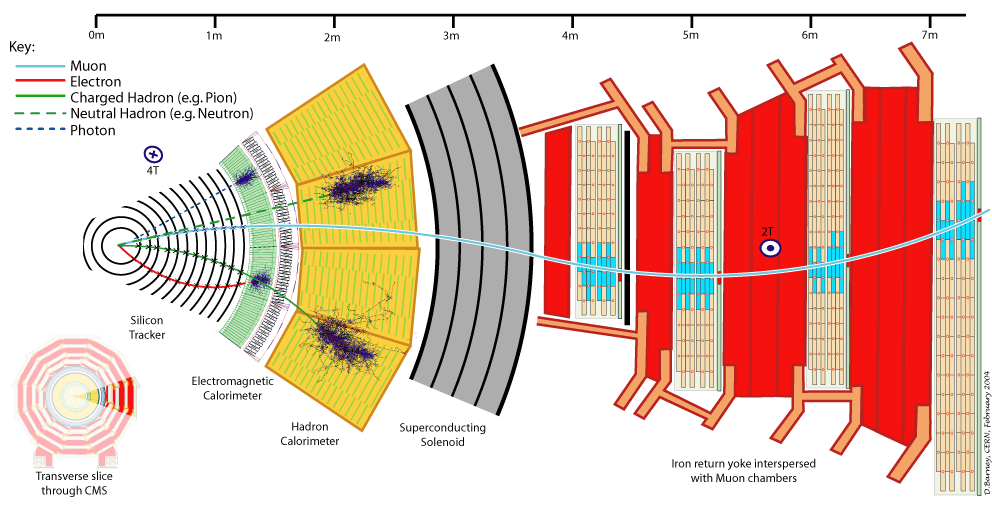
\includegraphics[width=0.95\textwidth]{tex/reco/fig/reco-cms.png}
  \caption{A cartoon schematic of the CMS detector, shown in the $r-\phi$ plane.
    The ideal interactions of muons, electrons, pions, neutrons, and photons 
    with various components of the detector are shown.
  }
  \label{fig:reco}
\end{figure}

The local reconstruction process takes digitized electronic 
signals called ``Digis'' as its input.  These Digis may
come from the real detector electronics or from a simulation
of those electronics.  The same local reconstruction algorithms
are used in either case, and the output objects are called ``RecHits''.
The global reconstruction process combines RecHits from various
modules of a single subdetector, but it does not combine information
from modules from different subdetectors.  To use muons as an example:
tracker tracks are created from tracker RecHits, and standalone
muon tracks are created from muon system RecHits, but global muon candidates
are not yet formed.
Finally, the higher-level reconstruction process combines RecHits from 
different subdetectors to produce higher-level objects, including
global muon candidates.  

All reconstruction processes are performed using the CMS software framework 
and the ROOT software package \cite{root-1,root-2,root-3},
which are based on the C++ and Python programming languages.
As mentioned in Section \ref{sec:trigger}, this is the same software framework
used by the HLT.
The reconstruction processes for various physics
objects are described in greater detail in the following subsections.
